%%%%%%%%%%%%%%%%%%%%%%%%%%%%%%%%%%%%%%%%%%%%%%%%%%%%%%%%%%%%%%%%%%%%%%
% Project Report 
%%%%%%%%%%%%%%%%%%%%%%%%%%%%%%%%%%%%%%%%%%%%%%%%%%%%%%%%%%%%%%%%%%%%%%


%%% Preamble
\documentclass[paper=a4, fontsize=11pt]{scrartcl}
\usepackage[T1]{fontenc}
\usepackage{fourier}

\usepackage[english]{babel}															% English language/hyphenation
\usepackage[protrusion=true,expansion=true]{microtype}	
\usepackage{amsmath,amsfonts,amsthm} % Math packages
\usepackage{amsthm}
\usepackage{amsmath,amssymb}
\usepackage{graphicx}	
\usepackage{url}


%%% Custom sectioning
\usepackage{sectsty}
\allsectionsfont{\centering \normalfont\scshape}


%%% Custom headers/footers (fancyhdr package)
\usepackage{fancyhdr}
\pagestyle{fancyplain}
\fancyhead{}											% No page header
\fancyfoot[L]{}											% Empty 
\fancyfoot[C]{}											% Empty
\fancyfoot[R]{\thepage}									% Pagenumbering
\renewcommand{\headrulewidth}{0pt}			% Remove header underlines
\renewcommand{\footrulewidth}{0pt}				% Remove footer underlines
\setlength{\headheight}{13.6pt}


%%% Equation and float numbering
\numberwithin{equation}{section}		% Equationnumbering: section.eq#
\numberwithin{figure}{section}			% Figurenumbering: section.fig#
\numberwithin{table}{section}				% Tablenumbering: section.tab#


%%% Maketitle metadata
\newcommand{\horrule}[1]{\rule{\linewidth}{#1}} 	% Horizontal rule

\title{
		%\vspace{-1in} 	
		\usefont{OT1}{bch}{b}{n}
		\normalfont \normalsize \textsc{Technical University of Denmark - DTU Compute -} \\ [20pt]
		\horrule{0.5pt} \\[0.4cm]
		\LARGE \textsc{[SuperStringWithExpansion]} Problem \\
		\horrule{2pt} \\[0.5cm]
}
\author{
		\normalfont 							
        Salik Lennert Pedersen \\
        Anders Holmgaard Opstrup \\
        Federico Bergamin \\ [-3pt]		\normalsize
}
\date{}



%%% Begin document
\begin{document}
\maketitle
\section{Description of the problem}
In \textsc{SuperStringWithExpansion} decision problem we have two different alphabet $\mathcal{\Sigma}$ and $\mathcal{\Gamma}$, where $\mathcal{\Gamma}=\{\gamma_1,...,\gamma_m\}$ contains $m$ symbol, a string $s$ which is made up of symbols that belongs to the  $\mathcal{\Sigma}$ alphabet (formally $s\in\mathcal{\Sigma^*})$, $k$ strings $t_1,...,t_k$, which is made up of symbols from both alphabets ($t \in (\Sigma \cup \Gamma)^*)$, and in the end, we have $m$ subsets $R_1,...,R_m \subseteq \mathcal{\Sigma^*}$. These subsets contain symbols of $\mathcal{\Sigma}$ alphabet, and as we can notice, they are as many as the symbols in the alphabet $\mathcal{\Gamma}$. That's because for each $\gamma_i$ there is a subset $R_i$. We can understand better this relation explaining the core of our problem. \newline
\noindent The output of the problem will be YES if exits a sequence of words $r_1\in R_1$, $r_2\in R_2$,...,$r_m\in R_m$, such that for all $1 \leq i \leq k$ the so-called \textit{expansion} $e(t_i)$ is substring of $s$; the expansion of a string $t_i$ consists in the replacement of every symbols $\gamma_j \in \mathcal{\Gamma}$ that appears in the string $t_i$ with its expansion, where the expansion of a symbol is defined as follow: $e(\gamma_j):=r_j$. That is, we have to choose for every symbol $\gamma_j\in \mathcal{\Gamma}$ a symbol $r_j\in R_j$, and we know that $r_j \in\mathcal{\Sigma^*}$. We have to replace the symbol $\gamma_j$ in each string $t_i$ with the symbol $r_j$ that was chosen. We have to do that for each $\gamma \in \mathcal{\Gamma}$. In this way, using these replacements, we are transforming our string $t_i$ in its expansion $e(t_i)$. \newline 
In the end we will obtain that every expansion-string is made up of symbols of the alphabet $\mathcal{\Sigma}$ as our string $s$. Hence, if every new constructed string $e(t_i)$ is a substring of $s$, the answer for our problem will be YES, otherwise NO.
\newline
In other words, the answer of our problem will be YES if there is a selection of the $r_i \in R_i$ such that, replacing each symbols $\gamma_i \in \Gamma$ with the respective symbol $r_i$ (we have to remember that for each $\gamma_i$ we have to chose one symbol from the subset $R_i \subseteq \Sigma^*$) in every string $t\in T$, where $|T|=k$, we will have that every new string that we obtain with this replacement is a substring of the string $s$. 
If a selection of $r_i \in R_i$ like this doesn't exist, the answer will be NO.

\subsection{Simple examples}
With the text of the problem we receive also some problem instances on the alphabets $\Sigma=\texttt{\{a,b,...,z\}}$, $\Gamma=\texttt{\{A,B,...,Z\}}$. The first line of the file contains the number k, which is the number of strigs $t$ we have. The second line contains the string $s$ and the following $k$ lines the strings $t_1,..., t_k$. Finally, the last lines (at most 26, the number of letters in the alphabet) start with a letter $\gamma_j\in \Gamma$ followed by a colon and the contents of the set $R_j$ belonging to the letter, where the elements of the set are separated by commas. Hence, we can clearly see that for each symbols $\gamma_i \in \Gamma$, in this case letter, there is a subset $R_i$ and in this subset we have to chose one symbol.
\newline
\\
\noindent For example: \newline
\\
\noindent\texttt{4} \\
\noindent \texttt{abdde} \\
\noindent \texttt{ABD} \\
\noindent \texttt{DDE} \\
\noindent \texttt{AAB} \\
\noindent \texttt{ABd} \\
\noindent \texttt{A:a,b,c,d,e,f,dd} \\
\noindent \texttt{B:a,b,c,d,e,f,dd} \\
\noindent \texttt{C:a,b,c,d,e,f,dd} \\
\noindent \texttt{D:a,b,c,d,e,f,dd} \\
\noindent \texttt{E:aa,bd,c,d,e} \\

\noindent In this example we can observe that there is NO possible selection of symbols $r_i$ such that every string $t$ would be a substring of \texttt{s=abdde}. In fact if we have a look to $t_2$=\texttt{DDE} and $t_3$=\texttt{AAB}, we can notice that they have the same structure, and in the same time in our string $s$ the only letter that is repeated twice is the \texttt{d}. So we conclude that \texttt{A=d} and \texttt{D=d}. Moreover from $t_4$=\texttt{ABd} we see that, since $t_4$ will be a substring, or \texttt{B=d} or \texttt{B=b}. If we try to choose our selection of $r_i$ following these rules, we can noticed that there is no possible solution, such that at the same time, all $e(t_i)$ are substring of $s$.

\section{\textsc{SuperStringWithExpansion} is in $\mathcal{NP}$}
We have to show and prove that our problem is in $\mathcal{NP}$. To do that we use the so called \textit{guess-verify algorithms} proof, so we have to start designing a deterministic algorithm A which takes as input a problem instance X and a random sequence R. \newline
\textbf{Important:} In this case, since we already use R to indicates the subset of the problem, we are going to call the random sequence with the capital letter \textbf{G}.

\begin{proof}
	We have to show that there is a polynomial \textit{p} and a randomized \textit{p}-bounded algorithm $A$ which satisfies the condition of the class $\mathcal{NP}$.  
	
	\begin{enumerate}
		\item Let $\Sigma$ be an alphabet and $\Gamma$ another alphabet. We know that $|\Gamma|=m$ (cardinality of the alphabet $\Gamma$ is $m$). Let $s$ be a string made up of symbols of $\Sigma^*$ and let $t_1,...,t_k$ be $k$ strings made up of symbols of $(\Sigma \cup \Gamma)^*$. Then let $R_1,...,R_m$ be subsets that contains symbols of $\Sigma^*$. So the first part of the input is:
		$$ X = (\Sigma,\Gamma,s,t_1,...,t_k,R_1,...,R_m) $$
		We could simplify this symbolism, considering the set $T=\{t_1,...,t_k\}$ and $R=\{R_1,...,R_m\}$. In this way we obtain that the first part of the input for our algorithm A now is:
		$$ X = (\Sigma,\Gamma,s,T,R) $$
        \begin{enumerate}
        	\item The random sequence $G$ consists of \textbf{integers} in the range $\{1,...,n\}$, where $n=max({|R_i|})$ for $1 \leq i \leq m$.
        	
        	\item Now on input $((\Sigma,\Gamma,s,T,R),\textbf{G})$, algorithm $A$ checks whether $G$ contains at least $m$ integers, and for every integer it has to check whether:
        	$$ int_j \leq |R_j| $$
        	which means that $A$ has to check if the integer contains in the position $j$, where $1 \leq j \leq m$, is less or equal than the cardinality of the subset $R_j$. The reason of that will be clear immediately. \newline
        	If $G$ is shorter, or the first $m$ integer don't satisfy the condition above, $A$ will return NO. Otherwise $A$ uses the first $m$ integers $g_1,...,g_m$ of $G$ to select a symbols in every subsets $R_1,...,R_m$. In this way:
        	$$ r_{g_i} \in R_i$$
        	That is, the integer $g_i$, which is in the position $i$ inside the random string $G$, indicates the position of the symbol that we have to choose inside the subset $R_i$. That's why it has to satisfy the condition above, in fact if the integer $g_i$ is greater than the cardinality of $R_i$ we are not able to select a symbol. 
        	
        	\item Now we have to choose an element for every subset $R_i$, where $1 \leq i \leq m$, and then using the expansion for the symbols of the alphabet $\Gamma$, we are able to "link" a letter $\gamma_i \in \Gamma$ with a symbol in $R_i$. (That's because for each letter $\gamma_i$ we have to choose one and only one symbol in the subset $R_i$, the $i$ is the same, because the subset is linked to the letter).
        	\begin{center}
        		$$\gamma_i \in \Gamma \Longrightarrow e(\gamma_i) = r_j \in R_i$$ \\
        		\noindent where $j=g_i$ of the string $G$
        	\end{center}
            Now we could substitute every letters $\gamma_i \in \Gamma$, $1\leq i \leq m$, which are in the $k$ strings $t$ with their expansion that we obtained thanks to the formula above. After that, we will have $k$ strings $e(t_i)$ (which are the expansion of our strings) made up of only symbols in $\Sigma^*$. \newline
            Then we have to check if every string that we obtain $e(t_l)$, $1\leq l\leq k$, is a substring of our string $s$. If every string is a substring the algorithm A returns YES, otherwise it returns NO.
        \end{enumerate}
        \item Now we have to show that the two conditions of the class $\mathcal{NP}$ are met:
        \begin{enumerate}
		   	\item Let us first assume that the true answer is YES, so there is a selection of symbols $r_1,...,r_m$ from the subsets $R_1,...,R_m$ such that, using the expansion for the symbols $\gamma \in \Gamma$ first, and then for the $k$ strings $t$, we will obtain that every string $e(t)$ (the expanded one) is a substring of $s$. So the symbols $r_1,...,r_m$ is our solution. That means, that our subsets $R_1,...,R_m$ contains one symbol each to expand $\gamma_1,...,\gamma_m \in \Gamma$ in the right way, and we have to choose exactly that symbol in every subset $R_i$. \newline
		   	Hence, there will be a string $G=g_1...g_m$ (which is the random string and contains the position of the element we will select) such that we will select the right symbol inside every subset $R$, so we are able to obtain that every string $e(t_i)$ is a substring of $s$. In this case if $G$ is given to $A$, $A$ will correctly return YES. Hence, there is a string of length at most $m$ which lead to a correct answer YES.
		   	To calculate the probability to obtain this string we try to see how to built this string that satisfy our problem: we show this probability in the two cases: the first, where all the subsets have exactly $n$ elements (which is useful to understand how change the probability in regard to the number of elements of the subsets and the number of the subsets) and the second, in which we consider every cardinality of the subset. We have to choose exactly one element in each subset, so our $g_i$ has to be the exactly position of the right symbols. In the first case for each $g_i$ we have to choose $1$ position between $n$, ans so we have: 
		   	\begin{center}
		   		$$G=g_1g_2...g_{m-1}g_m$$
		   		\textbf{P}[G is the right string]$= \underbrace{ {\left(\frac{1}{n}\right)\times ... \times \left(\frac{1}{n}\right)}}_\text{$m$ times} = \left(\frac{1}{n}\right)^m$
		   	\end{center}
	   	    Otherwise, if we want to use subset with no fixed cardinality, we have this probability:
		   	\begin{center}
		   		$$G=g_1g_2...g_{m-1}g_m$$
		   		\textbf{P}[G is the right string]$= \left(\frac{1}{|R_1|}\right)\times ... \times\left(\frac{1}{|R_m|}\right)$
		    \end{center}
	        We could see that this probability is small, especially if $n$ and $m$ are bigger, but it's positive. Hence, the first condition is satisfied.
	        \item Now, we assume that the true answer is NO, so there is no possible selection of symbols $r_1,...,r_m$ from $R_1,...,R_m$ such that every expanded-strings $e(t_i)$ are substring of $s$. In other words, for each random string $G$ we pass to $A$, there is no possible sequence of position $g_1...g_m$ such that let us select the right symbols to obtain that every expanded-strings $e(t_i)$ are substring of $s$. Hence, regardless the random string $G$, the algorithm $A$ will always answer NO in this case, so also the second condition is satisfied.
	   	\end{enumerate}
        \item Now we have to show that the running time of the algorithm $A$ that we've built is \textit{p}-bounded for some polynomial $p$. We could see that our algorithm have to:
	        \begin{itemize}
	        	\item check if $G$ contains at least $m$ integer: \textit{O(m)};
	        	\item for each integer check if the condition is satisfied: so for each integer has to calculate the cardinality of the subset $R_i$ related to the position $g_i$ and compare to the integer value. If we are going to use arrays we have to compare an integer to the \texttt{length} of the array. So it will be \textit{O(1)} for each element in $G$. For $m$ element it will be \textit{O(m)}; 
	        	\item select the exact element in $R_i$ using the position $g_i$ for every subset. If we will work with arrays we have to enter one cell, so \textit{O(1)}, but for all the letters of the alphabet $\Gamma$ is \textit{O(m $\times$ 1)} = \textit{O(m)};
	        	\item read all the $k$ strings and substitute all the $\gamma$ with their expansions. The worst case is when the length of the strings are almost $n$, so we have to read all the $k$ strings and substitute. If we think that a substitution is \textit{O(1)}, then it will be \textit{O(k $\times$ n)};
	        	\item in the end check if the all $k$ expanded-strings are substring of $s$. Using the simplest algorithm, we have that it will be \textit{O(n+q)}, where $n$ is the length of the string $s$ and $q$ the length of strings $t$. Hence, for all $k$ strings $t$ it will be \textit{O(k(n+q))}
	        \end{itemize}
        Therefore, we can see that our algorithm give the result in time:
        $$m+m+m+kn+k(n+q) = 3m+kn+k(n+q) $$
        In the worst case, we could have $n$ symbols in $\mathcal{\Gamma}$, and $n$ strings $t$, so the algorithm will be \textit{O($n^2$)}, which is polynomial.          
\end{enumerate}
\end{proof}

\section{\textsc{SuperStringWithExpansion} is $\mathcal{NP}-$complete}
In this section we are going to prove that our \textsc{SuperStringWithExpansion} problem is $\mathcal{NP}-$complete. 
\begin{proof}
     We could reduce from \textsc{Graph-3-Coloring}, which is a $\mathcal{NP}-$complete problem. In other words we have to define a \textit{transformation T}, that will create from each instance \textbf{X} of \textsc{Graph-3-Coloring} an instance of our problem \textsc{SuperStringWithExpansion}. \newline
     \\
     Let $G=(V,E)$ be the input graph for \textsc{Graph-3-Coloring}, where:
     \begin{center}
     	$V=\{v_1,v_2,...,v_n\}$ is the set of nodes \\
     	$E=\{e_1,e_2,...,e_k\}$ is the set of edges
     \end{center}
     we label the 3 colours red, blue, yellow in this way: $\{R,G,B\}$, and the transformation T works as follows. \newline
     Firstly we have to define two alphabets $\Sigma$ and $\Gamma$: we choose:
     \begin{center}
     	$\Sigma=\{R,G,B\}$ and $\Gamma=\{v_1,v_2,...,v_n\}$, that is, the nodes of the graph G.
     \end{center}
     Then, for each edge $e_i\in E$ we consider the two nodes that it links, and we create a string:
     \begin{center}
     	$t_i=v_a,v_b$ (where $v_a$ and $v_b$ are linked by $e_i$)  
     \end{center}
     In this way, our strings $t$ contains only letters of $\Gamma$. Hence, we satisfy the rule that $t \in (\Sigma \cup \Gamma)^*$ \newline
     Then we have to create the subsets relative to each letters of $\Gamma$, and in other words, to all nodes $v_1,...,v_n$.
     Therefore for each letter in $\Gamma$ we define:
     \begin{center}
     	$R_1=R_2=...=R_n=\{R,G,B\}$
     \end{center}
     In this way, using the structure of the SWE file to understand better, we obtain:
     \begin{center}
     	$v_1: \{R,G,B\}$ and this is $R_1$ \\
     	$v_2: \{R,G,B\}$ and this is $R_2$ \\
     	$.$ \\
     	$.$ \\
     	$.$ \\
     	$v_n: \{R,G,B\}$ and this is $R_n$
     \end{center}
     We could notice that $R_i \in \Sigma^*$ for $1 \leq i \leq n$. \newline
     In the end we have to define the string $s$, and we do like this:
     \begin{center}
        $s=BRGRBG$
     \end{center}	
     We could see that the running time of this transformation T is linear in the input size, in fact for each edge $e\in E$, it creates a string with two literal (the nodes that the edge links). Hence, in total it crates $|E|$ string of length 2. Then for each node $\{v_1,...,v_n\}$ it creates a subset with three element. Hence, we obtain $n$ subset of size two. In the end it creates a string $s$. \newline
     \\
     \noindent Now suppose that there is a true answer to our \textsc{Graph-3-Coloring} instance \textbf{X}, then for definition of the problem, there is a "3-colours assignment" to the vertices:
     \begin{center}
     	$\{v_1,v_2,...,v_n\} \rightarrow \{R,G,B\}$
     \end{center} 
     such that all adjacent nodes don't have the same colour. We claim that, then, there exists a selection of one element for each subset $R_1,...,R_n$, which are linked to the symbols $\{v_1,...,v_n\}$, such that after the substitution of $v_i$ with $r_i \in R_i$ (the chosen element) in all the strings $t$, we obtain that all the strings $t$ are substring of the string $s$. Consider that the expansion of each symbol $v_i \in \Gamma$ is equal to the colour of the "colour-assignment" to the vertices $v_i \in V$ that satisfies the \textsc{Graph-3-Coloring} problem instance. In other words every $v_i$ has the same colour of the node $v_i$, and in this way every symbol in $\Gamma$ could have one of these expansion: R,G or B. We could see that this will satisfy the rules, because our subsets $R_i = \{R,G,B\}$. \newline
     Because of the way we construct our strings $t$, which contain each one two adjacent nodes, we obtain that through the expansion and the substitution of the symbols in $\Gamma$, each strings $t$ have to be the form of:
     \begin{center}
     	$RG, RB, GB, GR, BG, BR$
     \end{center}
     That's because the "colour-assignment" satisfies the \textsc{Graph-3-Coloring} problem ans so every pair of adjacent nodes doesn't have the same colour. Hence, every string $t$ has to be substring of our string $s$, so we constructed a satisfying selection for the instance of \textsc{SuperStringWithExpansion}. \newline
     \\
     \noindent On the other hand, let us assume that there exists a selection of one element for each subset $R_1,...,R_n$, such that, after the expansion of each symbols in $\Gamma$ and its substitute inside the strings $t$, in this way:
     \begin{center}
     	$v_1 \rightarrowtail r_1\in R_1$ \\
     	$v_2 \rightarrowtail r_2\in R_2$ \\
     	$.$ \\
     	$.$ \\
     	$.$ \\
     	$v_n \rightarrowtail r_n\in R_n$ \\
     	where $R_1,...,R_n = \{R,G,B\}$
     \end{center}
     we obtain that all strings $t$ are substring of string $s$. We claim, then, that there exist a "colour-assignment" to the vertices of $G=(V,E)$, such that all adjacent nodes don't have the same colour. Because of the construction of our strings $t$, which represent all the pairs of adjacent nodes, if we have a YES answer to the \textsc{SuperStringWithExpansion} problem, it means that every string $t$ has one of these forms:
     \begin{center}
     	$RG, RB, GB, GR, BG, BR$
     \end{center}
     that's because, these are all the possible substring of length 2 of our string $s$.Hence, we can see that, since we have a satisfying selection, we cannot have a string $t$ that contains two equal literals. That means that every two adjacent nodes have different colours. Therefore we find also a satisfying "colour-assignment" for the \textsc{Graph-3-Coloring} problem. \newline
     \\
     That shows the we can reduce from \textsc{Graph-3-Coloring}, then our problem \textsc{SuperStringWithExpansion} is in $\mathcal{NP}$-complete. \newline
     \\
     \\
    \end{proof}
     \noindent These are two example about how our transformation works: in the first example there is a YES answer, in the second, instead, is not possible. 
     
    
     \begin{figure}[h]
     	\centering
     	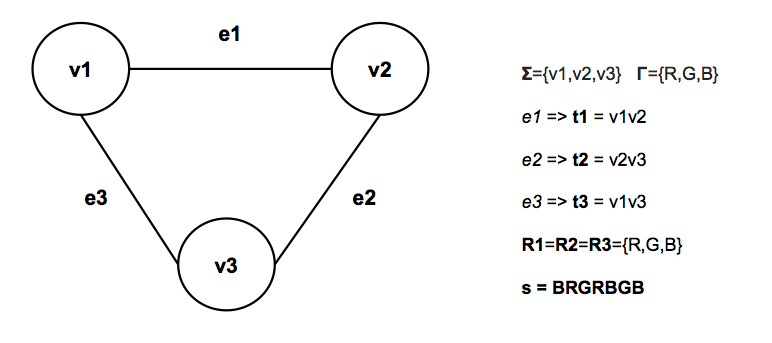
\includegraphics[scale=0.4]{imgs/graph1}
     	\caption{Example of a YES answer}\label{fig:1}
     \end{figure}
     \begin{figure}[h
     	]
     	\centering
     	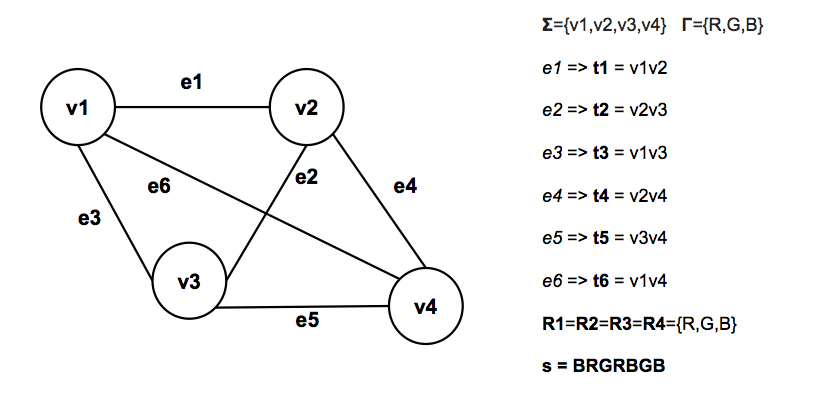
\includegraphics[scale=0.4]{imgs/graph2}
     	\caption{Example of a NO answer}\label{fig:1}
     \end{figure}



\section{Implementation of the decoder}
We have to implement a decoder that read a SWE files, which contains an instance of our \textsc{SuperStringWithExpansion} problems (where $\Sigma$ is the lower-case alphabet and $\Gamma$ the upper-case one), that check if these are written in a correctly way, and in particular rejected the files in which the subset $R_i$ are not specified in a proper way.  \newline
Our program has to read line to line the SWE file and check if everything is correct. Hence, we have to check these things:
\begin{itemize}
	\item the first line has to be a number, which represents the number of the strings $t$;
	\item the second line has to be a string made up of only lower-case characters, we cannot accept numbers, symbols and upper-case letters;
	\item each string $t$ has to be a string which could make up of both upper-case and lower-case letters, but we cannot accept numbers and symbols. Moreover, the length of the string $t$ has to be less or equal to the length of the string $s$;
	\item each subset has to begin with a capital letter followed by the column and then there has to be lower-case letter separated by the comma. We have to check if this "grammar" is respected, hence, we cannot accept symbols, blank spaces, upper-case letter except at the beginning. Moreover we have to check that there exists a subset for all the upper-case letter that appears on the strings $t$.
\end{itemize}
The program code (in Java) is attached in the project folder. 






%%% End document
\end{document}